%\section{Power Model} \label{sec:powermodel}
%Some of the main factors that contribute to the CPU power consumption are the dynamic power consumption, the short-circuit power consumption, and the power loss due to the transistor leakage current, \cite{Rauber2014, Goel2016, Du2017, Gonzalez1997}. The complexity of the circuits of modern processors makes it very difficult to consider all the components and interconnections. A viable approach for modeling the CPU's power draw is to model their building components, which are mainly made out of logic gates. Thus, modeling the power consumption can be resumed to model the logic gates and multiplying this by the total number of gates, reducing the complexity of the modeling process. %Although this is a huge simplification, it can still provide sufficient accuracy, bellow 5\%
%
%The mature technology to manufacture logic gates is CMOS. Nowadays it has been replaced by FINFET. In general, in these technologies, there are three main components of power dissipation \cref{eq:power_breakdown}. Namely, static power $P_{\rm static}$, dynamic power $P_{\rm dynamic}$, and leakage power $P_{\rm leak}$, that accumulated compose the total power draw.
%\begin{equation}
%P_{total}=P_{\rm static}+P_{\rm leak}+P_{\rm dynamic}
%\label{eq:power_breakdown}
%\end{equation}
%
%The dynamic power and leakage power behavior can be approximated by \cref{eq:power_dyn} and \cref{eq:power_leak} respectively~\cite{Sarwar1997, Butzen2007}.
%\begin{equation}
%P_{dynamic}=CV^2f,
%\label{eq:power_dyn}
%\end{equation}
%\begin{equation}
%P_{leak} \propto V,
%\label{eq:power_leak}
%\end{equation}
%where $C$ is the transistor capacitance, $V$ the voltage applied to the circuit and $f$ the switching frequency.
%
%Another common approximation is to expect a linear relationship between the voltage and the applied frequency~\cite{Usman2013ANoC} such that \ref{eq:f_v}
%\begin{equation}
%f \propto V.
%\label{eq:f_v}
%\end{equation}
%Thus, the proposed model for one processing core of a multi-core processor is derived by using (\cref{eq:power_dyn}), (\cref{eq:power_leak}) and (\cref{eq:f_v}) to rewrite (\cref{eq:total_power}) as the following equation \ref{eq:total_power}.
%\begin{equation}
%P_{total}(f)= c_1f^3+c_2f+c_3,
%\label{eq:total_power}
%\end{equation}
%where $c_1$, $c_2$, and $c_3$ are the model's parameters. Including the number of active cores $p$, the estimation of the power consumption of the whole processor becomes \ref{eq:power_final}:
%\begin{equation}
%P_{total}(f,p)= p(c_1f^3+c_2f)+c_3.
%\label{eq:power_final}
%\end{equation}
%
%\section{Performance Model} \label{sec:performancemodel}
%To model the application execution time, we consider a program as a set of instructions that are executed on a mean frequency $f$ with $c_k$ instructions per cycle. The time $T_f$ that this program will take to complete in at a given frequency is devised as follows.
%\begin{equation}
%T_f=\frac{I}{c_kf},
%\label{eq:freqrel}
%\end{equation}
%where $I$ is the total number of instructions and $ck$ the ratio of instructions per unit of time.
%
%The next step is to include the number of cores in the equation. Amdahl's law, described in the equation \ref{eq:amdahl}, gives the theoretical background for that, it describes the speedup in latency of the execution of a task at a fixed workload.
%\begin{equation}
%S=\frac{T_s}{T_P}=\frac{1}{1-w+\frac{w}{p}},
%\label{eq:amdahl}
%\end{equation}
%where $S$ is the theoretical speedup of the execution of the whole task, $w$ s the proportion of execution time that the part benefiting from improved resources originally occupied, $p$ is the speedup of the part of the task that benefits from improved system resources. Combining this with \cref{eq:freqrel}, the parallel time at frequency $f$ can be written as:
%\begin{equation}
%T_p=\frac{T_s}{S}=\frac{T_f}{\frac{1}{1-w+\frac{w}{p}}}.
%\label{eq:parallel_time}
%\end{equation}
%
%Then, we write the execution-time equation of the program as a function of frequency, the number of cores and parallel proportion as \ref{eq:performance} and subsequently \ref{eq:performance_2}:
%\begin{equation}
%T(f,p)=\frac{I}{ \frac{c_kf}{1-w+\frac{w}{p}} },
%\label{eq:performance}
%\end{equation}
%\begin{equation}
%% T(f,p)=\frac{d_1 (1-w+\frac{w}{p}) }{f}
%T(f,p)=\frac{d_1(p-wp+w)}{fp}.
%\label{eq:performance_2}
%\end{equation}
%
%Finally, we include the input size so that the application is fully characterized, in \cite{Oliveira2018ApplicationCores} it was shown that generally this can be described with an exponential, as presented in \cref{eq:performance_final}.
%\begin{equation}
%% T(f,p)=\frac{d_1 (1-w+\frac{w}{p}) }{f}
%T(f,p,N)=\frac{d_1N^{d_2}(p-wp+w)}{fp},
%\label{eq:performance_final}
%\end{equation}
%where $d_1$ and $w$ are constants that depend on the application. This equation can describe the behavior of the execution time at any input $N$, frequency $f$ and active cores $p$.
%
%\section{Energy Model} \label{sec:energymodel}
%Combining the output of the power model described in~\cref{sec:powermodel} and the characterization of the application performance described in \cref{sec:performancemodel}, the total energy can be modeled as:
%\begin{equation}
%E(f,p,N)=P(f,p)\times{\rm T}(f,p,N),
%\label{eq:en_combination}
%\end{equation}
%where $P(f,p,s)$ is the total power modeled by~\cref{eq:power_final}, ${T}(f,p,N)$ is the execution time estimated by the \ref{eq:performance_final}, $f$ is the frequency, $p$ is the number of active cores, $s$ is the number of sockets, and $N$ is the input size. The final equation can be written as:
%\begin{equation}
%% E(f,p)=\frac{d_1((c_1f^3+c_2f)p+c_3)(1-w+\frac{w}{p}) }{f}
%E(f,p,N)=\frac{d_1N^{d_2}(p-wp+w)(p(c_1f^3+c_2f)+c_3)}{fp}.
%\label{eq:en_final}
%\end{equation}
%
%%%%%%%%%%%%%%%%%%%%%%%%%%%%%%%%%%%%%%%%%%%
%
%\section{Experimental validation} \label{sec:experimentalvalidation}
%In this section, the result of the models presented in~\cref{sec:powermodel} and~\cref{sec:performancemodel} were validated with a benchmark specific for multi-core architectures. The results were then compared with a machine learning approach, Support Vector Regression (SVR)~\cite{Smola2004}, to contrast the accuracy and overhead obtained with each case.
%
%\subsection{Case-Study Applications} \label{sec:casestudyapplication}
%The PARSEC parallel benchmark suite, version 3.0~\cite{Bienia2008}, OpenMC \cite{Romano2015OpenMC:Development} and LINPACK (HPL) \cite{Dongarra1988TheExplanation}, were chosen as cases of study. The PARSEC benchmark focus on emerging workloads and were designed to be representative of the next generation shared-memory programs for chip-multiprocessors. It covers an ample range of areas such as financial analysis, computer vision, engineering, enterprise storage, animation, similarity search, data mining, machine learning, and media processing. The OpenMC and the LINPACK applications are two classical HPC program.
%
%\subsection{Case-Study Architecture} \label{sec:casestudyarchitecture}
%The experiments were executed in one computer node equipped with two Intel Xeon E5-2698 v3 processors with sixteen cores each and two hardware threads for each core. The maximum non-turbo frequency is 2.3GHz, and the total physical memory of the node is 128GB (8$\times$16GB). Turbo frequency and hardware multi-threading were disabled during all experiments. The operating system used was Linux CentOS 6.5, kernel 4.16. The overview of the architecture is shown in figure \ref{fig:architecture}.
%\begin{figure}[h]
%	\centering
%	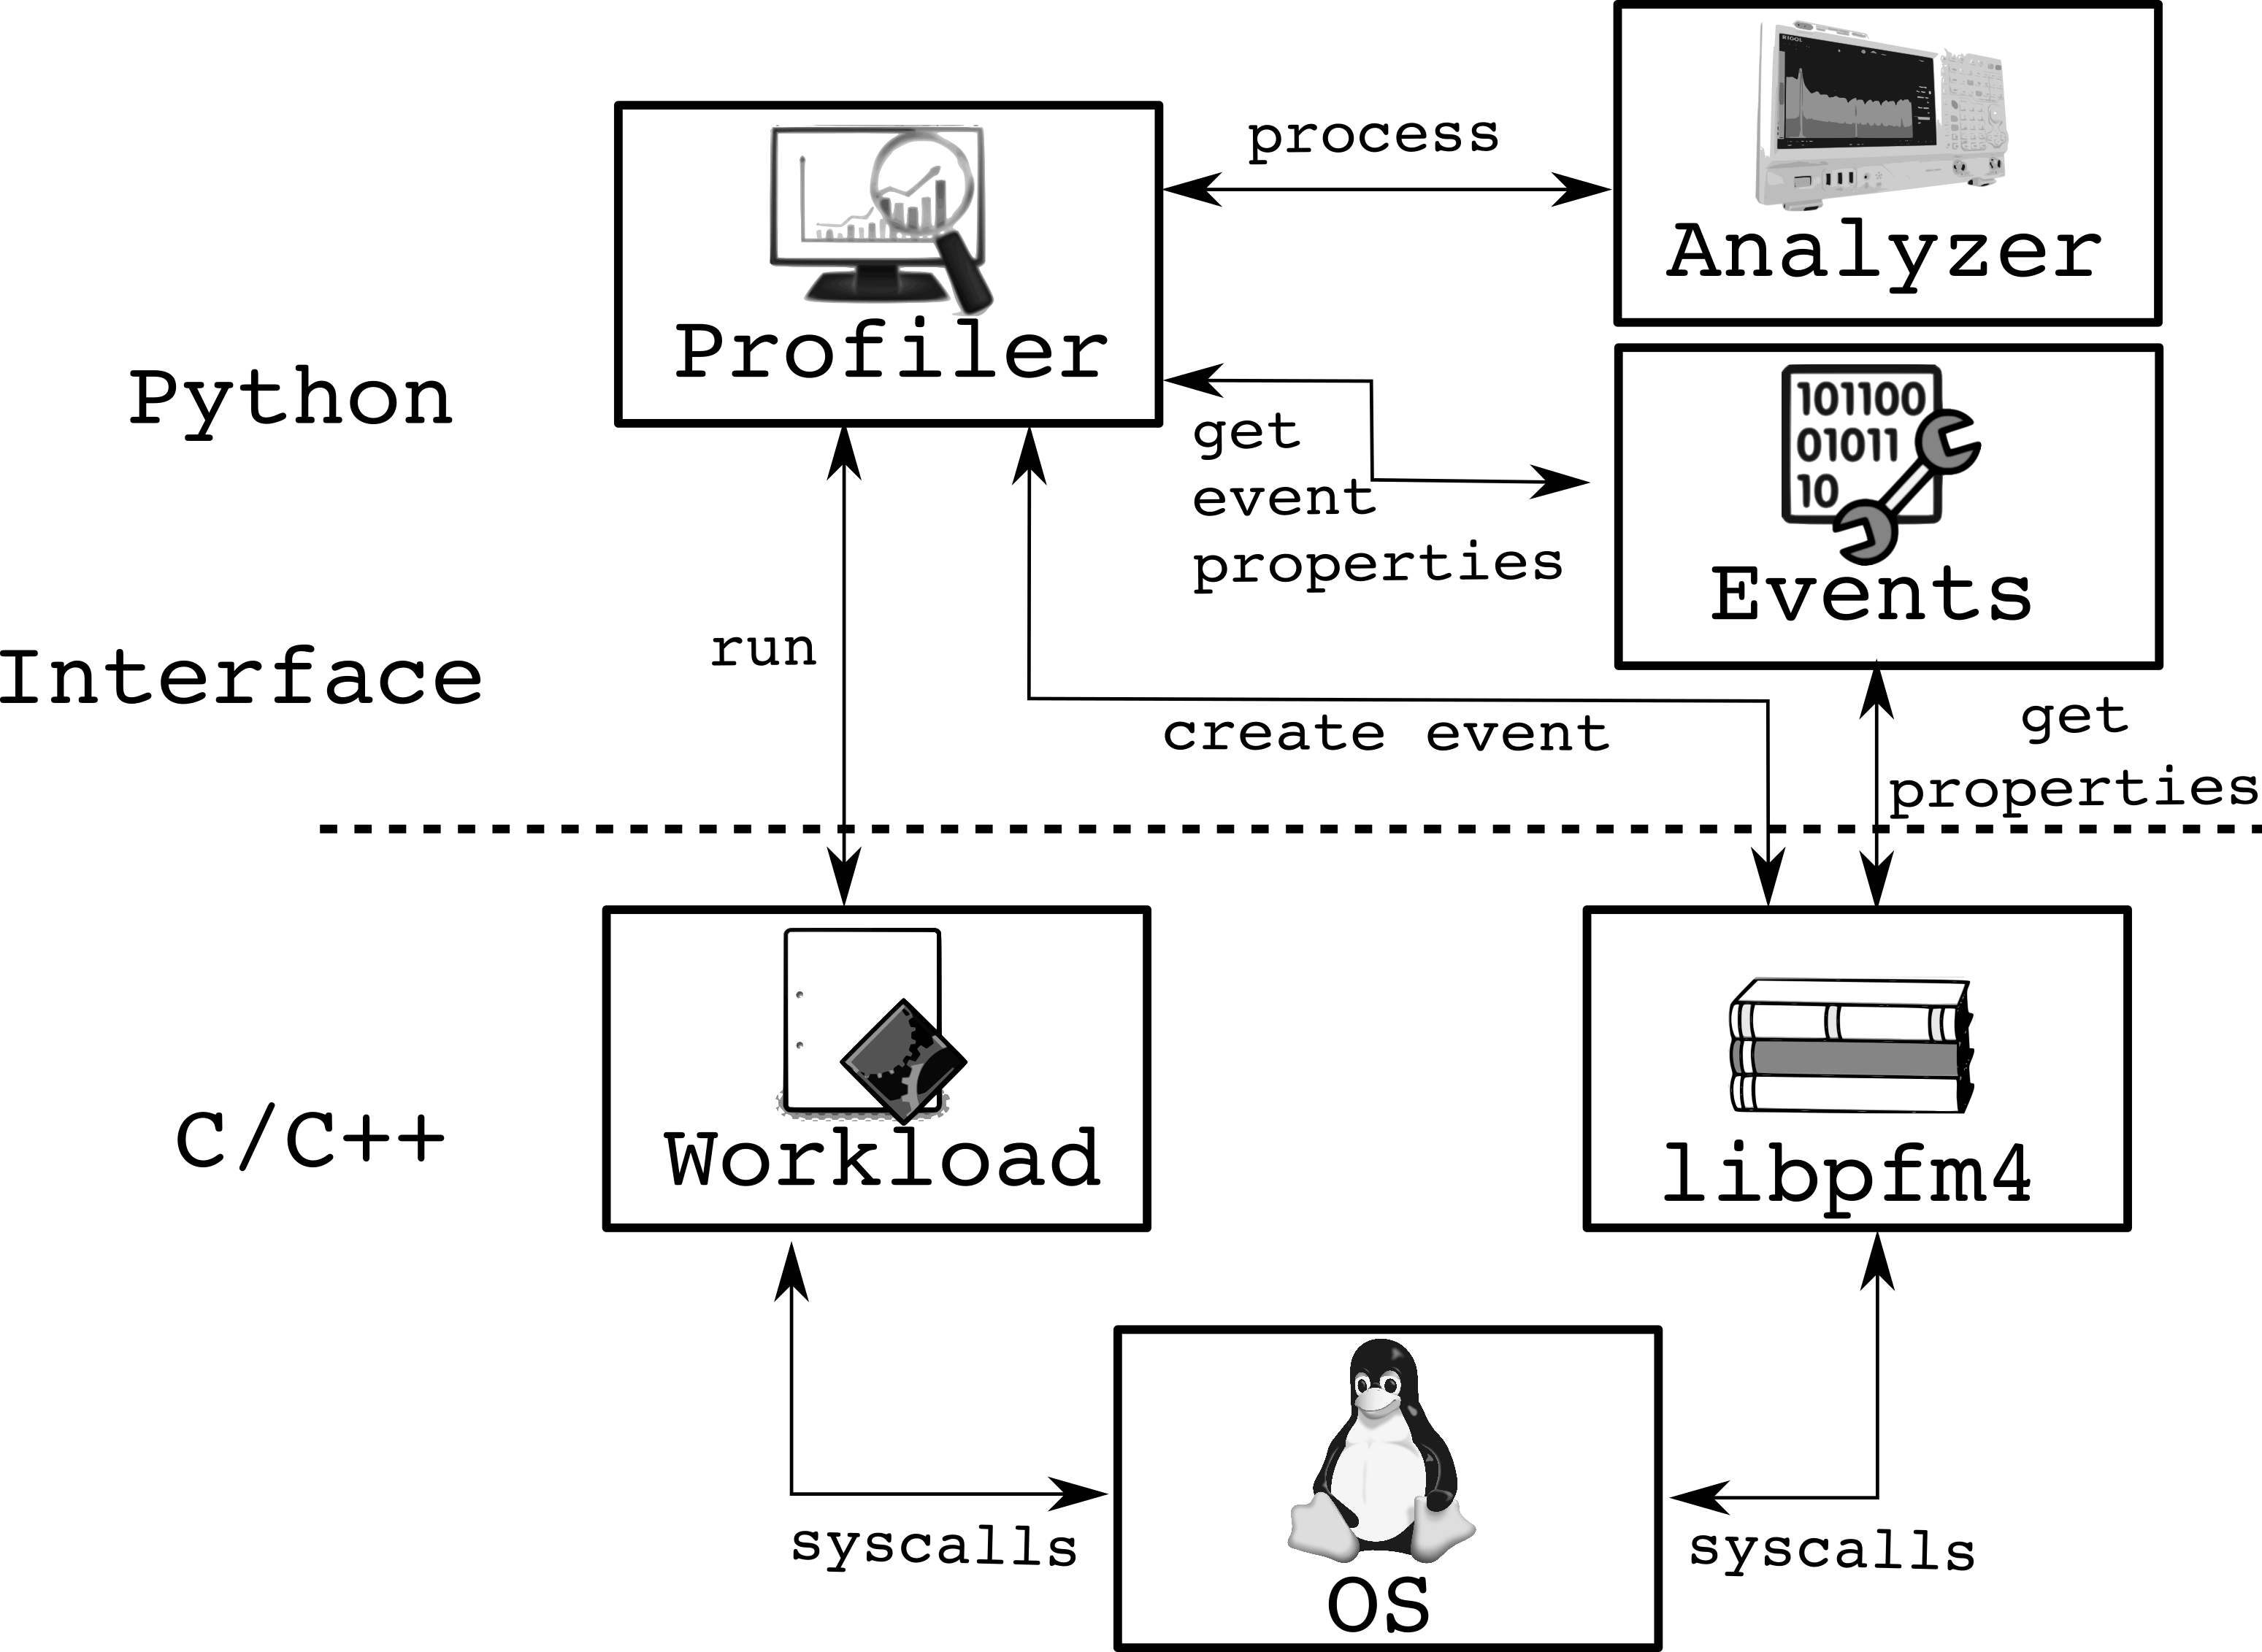
\includegraphics[width=\columnwidth]{models/models/figures/architecture.png}
%	\caption{Node architecture, the image was made with lstop application}
%	\label{fig:architecture}
%\end{figure}
%
%The Linux kernel has many different policies for power management depending on the driver. On the default driver the acpi-cpufreq, the options are:
%\begin{itemize}
%	\item Powersave
%	\item Performance
%	\item Ondemand
%	\item Conservative
%	\item Userspace
%\end{itemize}
%In this work, the frequency control was performed using the Userspace governor, and the core control was accomplished by modifying the appropriate system files with the default CPU-hotplug driver.
%
%This architecture is equipped with Intelligent Platform Management Interface (IPMI), which is a set of interfaces that allow out-of-band management of computer systems and platform-status monitoring through local network~\cite{Schwenkler2006IntelligentInterface}. It can monitor variables and resources such as the system's temperature, voltage, fans, and power supplies, with independent sensors attach to the hardware.
%
%\subsection{Fitting the Models} \label{sec:fitting}
%To find the parameters of the equation \ref{eq:en_final}, 10 random configurations of frequencies (f), cores (p) and inputs (N) were chosen from the range $1<=p<=32$, $1.2<=f<=2.2$ and $1<=N<=5$ respectively. The application ran with each configuration chosen and the results of energy and time were collected. The application's input was chosen in such a way that they increase workload linearly to the smallest workload to the biggest workload so that most of the input space is covered~\cite{Oliveira2018ApplicationCores}. For each configuration, samples of the power were collected using IPMI every 1 second. This sampling rate was chosen because the order of magnitude of the mean run time of the applications is minutes. Therefore, this rate provides enough samples to measure average power. Additionally, timestamps and the total run time were collected. The total energy spent on each configuration is estimated by integrating the power samples over time.
%
%From the sampled data, the arguments of the model can be estimated.  For the equation, this results in an optimization problem of finding the parameters that minimize the total distance between the estimated values and the measured values. To solve this minimization problem, non-linear least squared was applied.
%
%The python library scikit-learning was used as the SVR implementation~\cite{PedregosaF.VaroquauxG.GramfortA.2011Scikit-learn:Python}.The SVR was trained using the same data of the equation with a grid search used to find the best kernel function and the best values for the hyper-parameters penalty for the wrong ($C$) and ($\gamma$). For this data, the best function was the Radial Base Function (RBF) and the hyper-parameters were $C=10\times10^3$ and $\gamma=0.5$. 
%
%\subsection{Measured versus Modeled Energy} \label{sec:measuredversusmodeledenergy}
%To validate the proposed energy model, all possible configurations were tested varying the cores in a range of $1<=p<=32$, the frequency in $1.2<=f<=2.2$ and input in $1<=N<=5$. Then, the mean absolute error was computed as the difference between the estimated values and the measured values according to the following equation.
%\begin{equation}
%MAE = \frac{1}{N} \sum_i^N \frac{|y_{\rm estimated}-y_{\rm measured}|}{y_{\rm measured}}.
%\label{eq:mae}
%\end{equation}
%
%Figures \ref{fig:en_eq_black}, \ref{fig:en_eq_canneal}, \ref{fig:en_eq_dedup}, and~\ref{fig:en_eq_rtview} plot the measured and modeled energy consumption for some of the applications modeled. There show some of the possible shapes that the model can assume while varying the number of active cores, operating frequency, and input size.
%\begin{figure}[ht]
%	\centering
%	
%	\begin{subfigure}[b]{0.48\textwidth}
%		\centerline{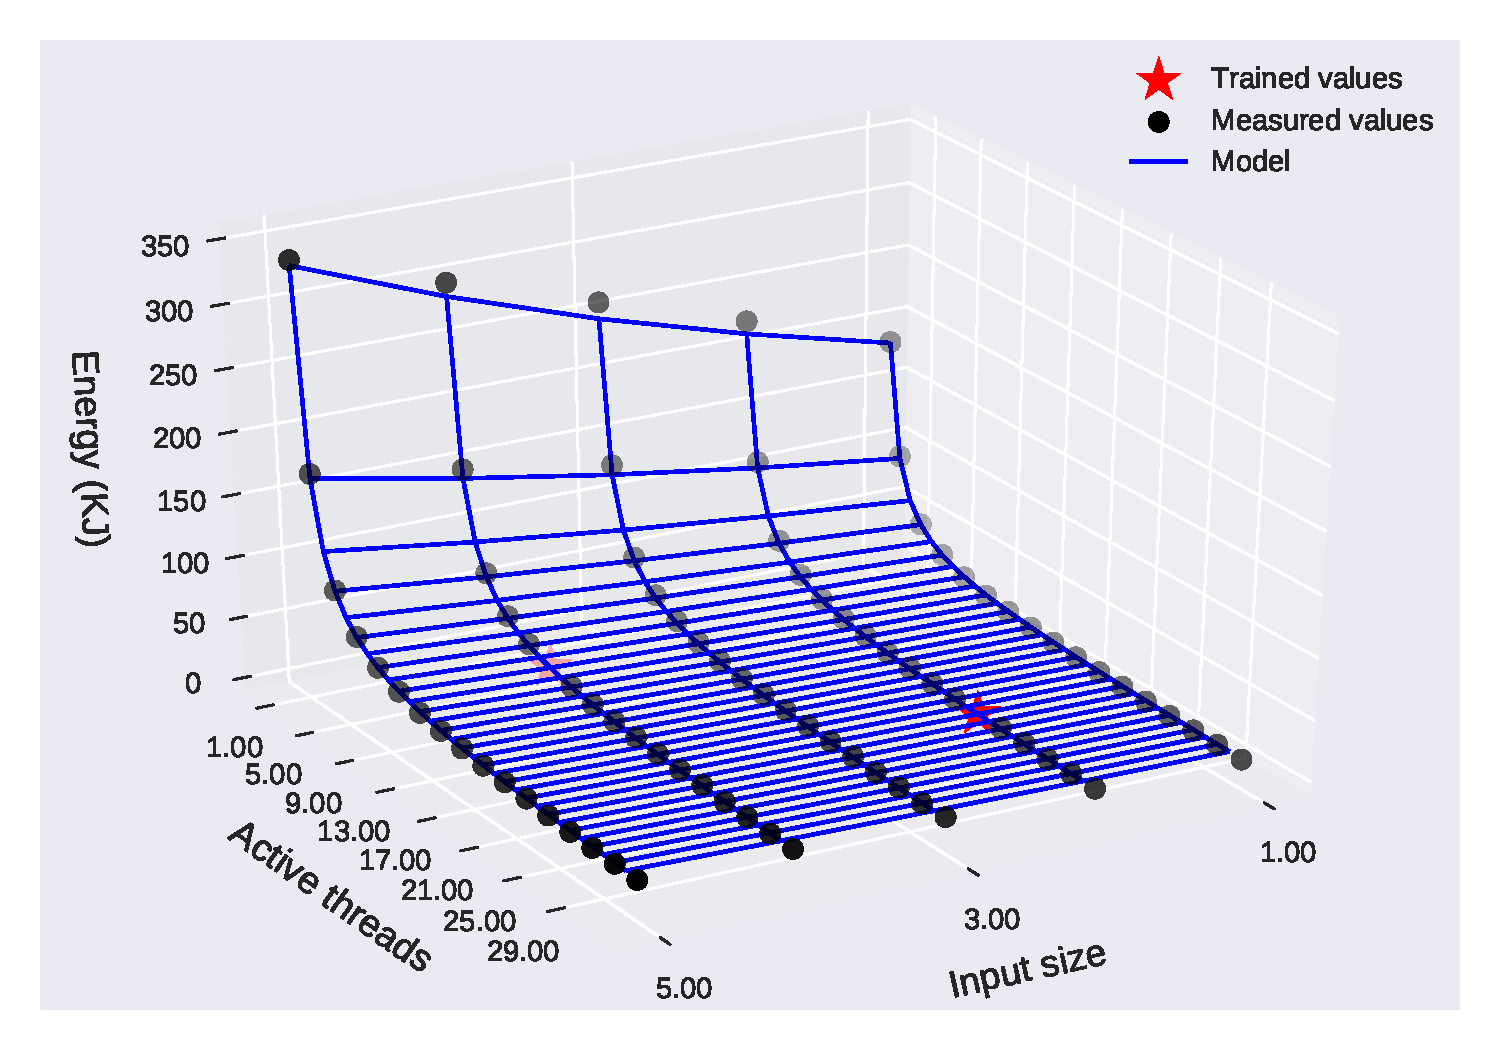
\includegraphics[width=\columnwidth]{models/models/figures/energy/completo_black_5.png}}
%		\caption{Blackscholes}
%		\label{fig:en_eq_black}
%	\end{subfigure}
%	%
%	\begin{subfigure}[b]{0.48\textwidth}
%		\centerline{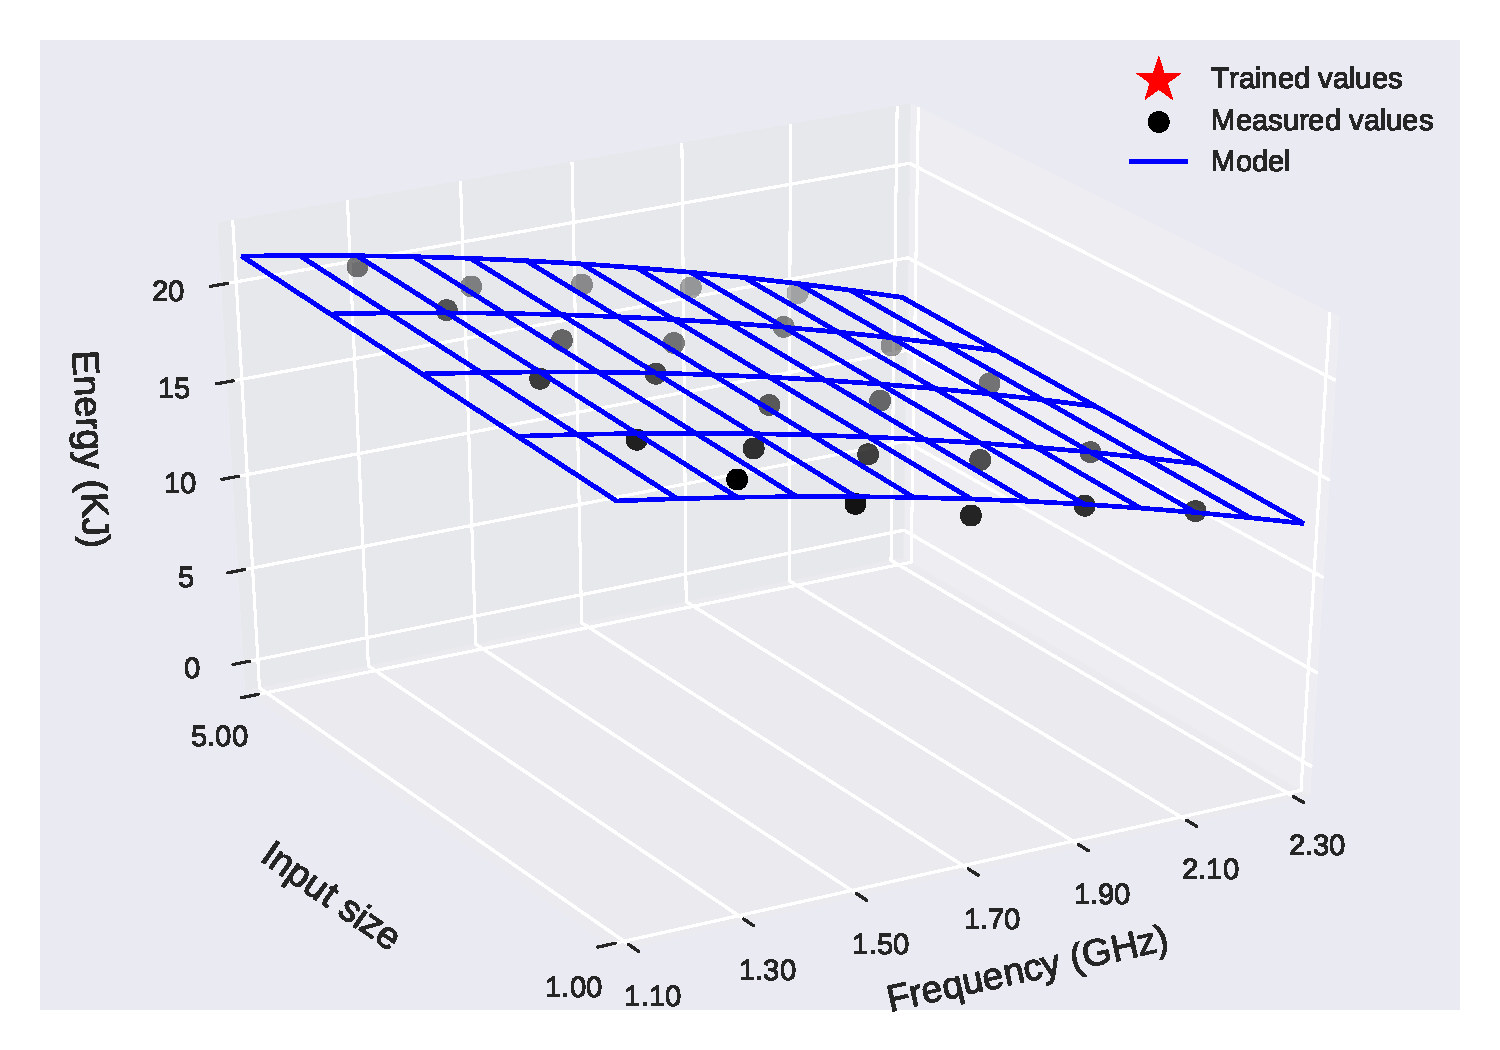
\includegraphics[width=\columnwidth]{models/models/figures/energy/completo_canneal_1.png}}
%		\caption{Canneal}
%		\label{fig:en_eq_canneal}
%	\end{subfigure}
%	
%\end{figure}
%
%\begin{figure}[ht]
%	\centering
%	
%	\begin{subfigure}[b]{0.48\textwidth}
%		\centerline{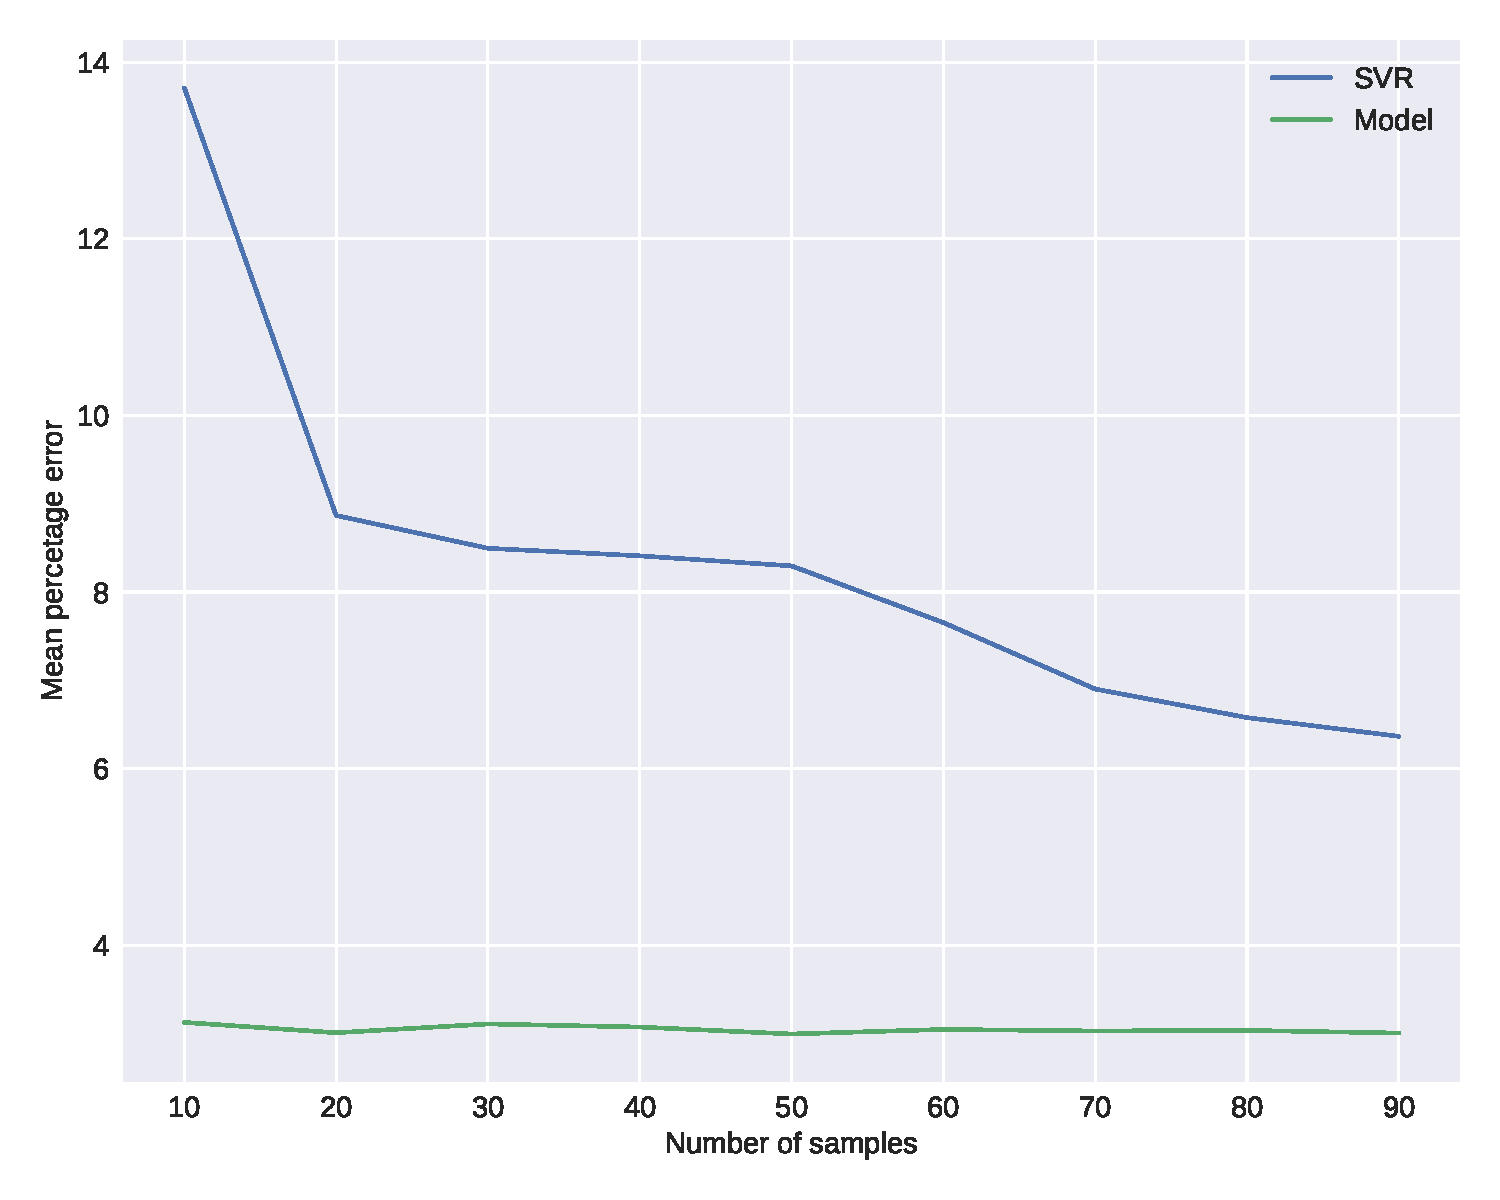
\includegraphics[width=\columnwidth]{models/models/figures/energy/completo_dedup_4.png}}
%		\caption{Dedup}
%		\label{fig:en_eq_dedup}
%	\end{subfigure}
%	%
%	\begin{subfigure}[b]{0.48\textwidth}
%		\centerline{\includegraphics[width=\columnwidth]{models/models/figures/energy/completo_rtview_4.png}}
%		\caption{Raytrace}
%		\label{fig:en_eq_rtview}
%	\end{subfigure}
%\end{figure}
%
%The validation results for each application trained with 10 random configurations are displayed in the figure \ref{fig:mae_svr_eq} and the raw MAE values in the table~\ref{tab:mae_svr_eq}.
%
%\begin{figure}[ht]
%	\includegraphics[width=\columnwidth]{models/models/figures/mae_svr_eq.png}
%	\caption{Comparison mean absolute error between the proposed model and SVR}
%	\label{fig:mae_svr_eq}
%\end{figure}
%
%\begin{table}[ht]
%	\centering
%	\begin{tabular}{|c|c|c|}
%		\hline
%		Application  & Model & SVR   \\ \hline
%		Ferret       & 5.25     & 12.49  \\ \hline
%		Raytrace     & 6.36     & 11.95  \\ \hline
%		Fluianimate  & 2.44     & 22.90  \\ \hline
%		x264         & 8.28     & 15.33  \\ \hline
%		Vips         & 7.54     & 10.80  \\ \hline
%		Swaptions    & 6.54     & 18.57  \\ \hline
%		Canneal      & 3.12     & 6.13   \\ \hline
%		Dedup        & 8.85     & 13.70  \\ \hline
%		Freqmine     & 2.44     & 3.24   \\ \hline
%		Blackscholes & 2.18     & 11.00  \\ \hline
%		HPL          & 7.47     & 12.75  \\ \hline
%		Bodytrack    & 16.98    & 34.12  \\ \hline
%		Openmc       & 11.15    & 24.34  \\ \hline
%	\end{tabular}
%	\caption{Comparison mean absolute error between the proposed model and SVR}
%	\label{tab:mae_svr_eq}
%\end{table}
%
%\subsection{Overhead on training}
%It is known that machine learning is data-driven, in that sense the results obtained using only 10 configurations could be improved, but how about the analytical model? To answer that question the proposed model and SVR were trained also with varying the number of configurations. Comparing the MAE and the amount of energy needed for each model. The figure \ref{fig:overhead_ferret}, \ref{fig:overhead_vips} show some of this comparisons for an individual application, while figure \ref{fig:overall_train} show the overall results for all applications.
%
%\begin{figure}[ht]
%	\centering
%	\begin{subfigure}[b]{0.45\textwidth}
%		\centerline{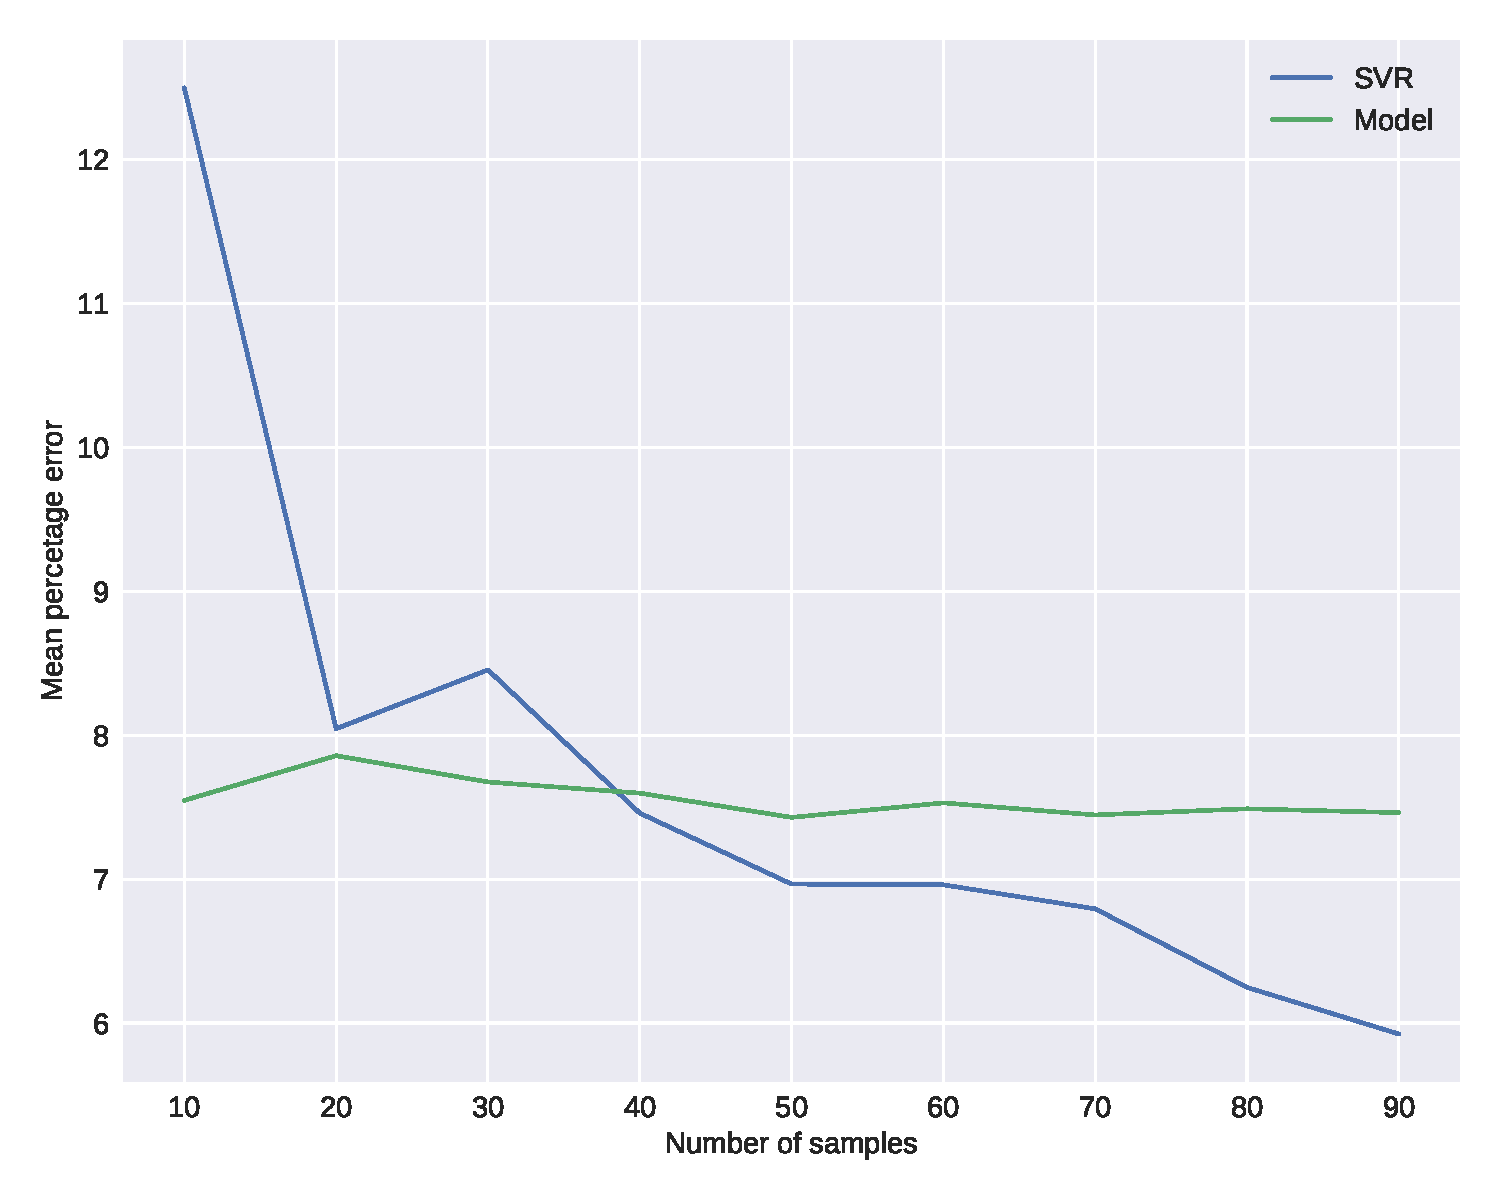
\includegraphics[width=\columnwidth]{models/models/figures/overhead/completo_ferret_4.png}}
%		\caption{MAE for Ferret}
%		\label{fig:overhead_ferret}
%	\end{subfigure}
%	%
%	\begin{subfigure}[b]{0.45\textwidth}
%		\centerline{\includegraphics[width=\columnwidth]{models/models/figures/overhead/completo_vips_4.png}}
%		\caption{MAE for Vips}
%		\label{fig:overhead_vips}
%	\end{subfigure}
%	\caption{MAE showing the that for the model is almost constant while for the SVR there are different crossing points for the lowest error}
%\end{figure}
%
%The analytical model demonstrates to be very stable, not changing a lot as more data are added, while the SVR keeps reshaping to adapt to the data. This reflects in the analytical model error being almost constant while the SVR drops meeting at some point.
%
%The figure \ref{fig:overall_train} present the overall results, computing the mean energy and MAE for all applications.
%
%\begin{figure}[ht]
%	\centering
%	\begin{subfigure}[b]{0.45\textwidth}
%		\centerline{\includegraphics[width=\columnwidth]{models/models/figures/overhead/overall_energy.png}}
%		\caption{Average energy spent over all applications}
%		\label{fig:overall_overhead}
%	\end{subfigure}
%	%
%	\begin{subfigure}[b]{0.45\textwidth}
%		\centerline{\includegraphics[width=\columnwidth]{models/models/figures/overhead/overall_mae.png}}
%		\caption{Average MAE over all applications}
%		\label{fig:overall_energy}
%	\end{subfigure}
%	\caption{Overall results for energy and MAE for each train size}
%	\label{fig:overall_train}
%\end{figure}
%
%The meeting point of the MAE for the SVR and the proposed model can be extracted from  \ref{fig:overall_overhead}. There it shows that approximately at 90 configurations the SVR starts to have a smaller error the cost of that is the linear increase in energy spent on training. The increase in energy of about $10\times$ can be observed in figure \ref{fig:overall_energy}.
%
%\subsection{Performance penalty}
%
%\subsection{Time to compensate energy spent on training}

\subsection{Power Model} \label{sec:powermodel}
The complexity of the modern processor's circuits makes it very difficult to consider all the components and interconnections. A viable approach for modeling the CPU's power draw is to model their building components, mainly made out of logic gates. Thus, modeling the power consumption can be resumed to model the logic gates and multiplying this by the total number of gates, reducing the complexity of the modeling process.

The mature technology to manufacture logic gates is CMOS. Nowadays, it has been replaced by FINFET. In general, in these technologies, there are three main components of power dissipation \cite{Rauber2014, Goel2016, Du2017, Gonzalez1997},  namely, static power $P_{\rm static}$, dynamic power $P_{\rm dynamic}$, and leakage power $P_{\rm leak}$, that accumulated compose the total power draw.
% \begin{equation}
% P=P_{\rm static}+P_{\rm leak}+P_{\rm dynamic}.
% \label{eq:power_breakdown}
% \end{equation}

The dynamic power and leakage power behavior can be approximated by \cref{eq:power_dyn} and \cref{eq:power_leak}, respectively, as shown by Sarwar et al. and Butzen et al~\cite{Sarwar1997, Butzen2007}.
\begin{equation}
P_{dynamic}=CV^2f,
\label{eq:power_dyn}
\end{equation}
\begin{equation}
P_{leak} \propto V,
\label{eq:power_leak}
\end{equation}
where $C$ is the load capacitance, $V$ the voltage applied to the circuit and $f$ the switching frequency.

Another common approximation is to expect a linear relationship between the voltage and the applied frequency~\cite{Usman2013ANoC} such that:
\begin{equation}
f \propto V,
\label{eq:f_v}
\end{equation}
Thus, the proposed model for one processing core of a multi-core processor is derived by using \cref{eq:power_dyn}, \cref{eq:power_leak} and \cref{eq:f_v} to write \cref{eq:total_power}.
\begin{equation}
P(f)= c_1f^3+c_2f+c_3,
\label{eq:total_power}
\end{equation}
where $c_1$ $c_2$, and $c_3$ are the model's parameters associated with the dynamic, leakage and static power aspects, respectively. Including the number of active cores $p$, the proposed estimation of the power consumption of the whole processor becomes \cref{eq:power_final}
\begin{equation}
P(f,p)= p(c_1f^3+c_2f)+c_3,
\label{eq:power_final}
\end{equation}

\subsection{Performance Model} \label{sec:performancemodel}
To model the application execution time, we consider a program as a set of instructions executed on a mean frequency $f$ with $c_k$ instructions per cycle. The time $T_f$ that this program will take to complete at a given frequency is devised as follows:
\begin{equation}
T_f=\frac{I}{c_kf},
\label{eq:freqrel}
\end{equation}
where $I$ is the total number of instructions and $c_k$ the ratio of instructions per unit of time.

The next step is to include the number of cores in the equation. Amdahl's law \cite{Amdahl1967ValidityCapabilities}, described in \cref{eq:amdahl}, gives the theoretical background for that. It describes the speedup in latency of the execution of a task at a fixed workload.
\begin{equation}
S=\frac{T_s}{T_p}=\frac{1}{1-w+\frac{w}{p}},
\label{eq:amdahl}
\end{equation}
where $T_s$ is the serial time, $T_p$ the parallel time, $S$ is the theoretical speedup of the execution of the whole task, $w$ is the proportion of the execution time that benefits from improving system resources, and $p$ is the part of the task that benefits from improved system resources. Combining this with \cref{eq:freqrel}, the parallel time at frequency $f$ can be written as:
\begin{equation}
T_p=\frac{T_s}{S}=\frac{T_f}{\frac{1}{1-w+\frac{w}{p}}},
\label{eq:parallel_time}
\end{equation}

We can then write the equation of the program execution time as a function of frequency, number of cores and parallelism  as \cref{eq:performance} and subsequently derive \cref{eq:performance_2}:
\begin{equation}
T(f,p)=\frac{I}{ \frac{c_kf}{1-w+\frac{w}{p}} },
\label{eq:performance}
\end{equation}
\begin{equation}
T(f,p)=\frac{d_1(p-wp+w)}{fp},
\label{eq:performance_2}
\end{equation}
where $d_1$ is a constant.

Finally, to fully characterize the application, a parameter representing the application's workload, called input size $N$, is introduced, representing the number of basic operations need to complete a problem \cite{Kumar1994AnalyzingArchitectures}. In Oliveira et al. \cite{Oliveira2018ApplicationCores}, they showed that this parameter could generally be described as exponential. Therefore the proposed performance model is presented in \cref{eq:performance_final}. This resulting equation can describe the behavior of the execution time of a program for an input $N$, frequency $f$, and active cores $p$:
\begin{equation}
T(f,p,N)=\frac{d_1N^{d_2}(p-wp+w)}{fp},
\label{eq:performance_final}
\end{equation}
where $d_1$, $d_2$ and $w$ are constants that depend on the application. 

\subsection{Energy Model} \label{sec:energymodel}
Combining the power model output described in~\cref{sec:powermodel} and the characterization of the application performance described in \cref{sec:performancemodel}, the total energy can be modeled as:
\begin{equation}
E(f,p,N)=P(f,p)\times{\rm T}(f,p,N),
\label{eq:en_combination}
\end{equation}
where $P(f,p)$ is the total power modeled by~\cref{eq:power_final}, ${T}(f,p,N)$ is the execution time estimated by the \cref{eq:performance_final}, $f$ is the frequency, $p$ is the number of active cores, and $N$ is the input size. The final equation can be written as:
\begin{equation}
E(f,p,N)=\frac{d_1N^{d_2}(p-wp+w)(p(c_1f^3+c_2f)+c_3)}{fp}.
\label{eq:en_final}
\end{equation}

%%%%%%%%%%%%%%%%%%%%%%%%%%%%%%%%%%%%%%%%%%